\documentclass[12]{article}

\usepackage{amsmath}
\usepackage{enumerate}
\usepackage{fancyhdr}
\usepackage{color}
\usepackage{listings}
\usepackage{graphicx}
\usepackage{hyperref}
\usepackage[margin=1in]{geometry}
\usepackage[default]{sourcesanspro}
\usepackage{sourcecodepro}

\definecolor{lightgray}{gray}{0.5}
\pagestyle{fancy}

\title{CISC 360 Project}
\author{Ryan McKenna, Matthew Paul, Niko Gerassimakis,\\ Neil Duffy, James Kerrigan}

\lstset{language=C, frame=single, showstringspaces=false}

\begin{document}
\maketitle

\section{Introduction}

LU Factorization is the most common technique used to solve systems of linear equations.  It is most useful when solving a dense linear system and is only appropriate when the system is square.  It works by decomposing a square matrix $A$ into an lower triangle matrix, $L$ and an upper triangular matrix $U$ such that 

$$ A = LU $$

\subsection{Impact}

Triangular matrices have a number of nice properties that make them easier to work with.  For example, if $ T $ is a triangular matrix, then you can solve the equation

$$ T x = b $$ 

in $O(n^2)$ time, as opposed to $O(n^3)$ for full matrices.  Computationally, this means we can solve $k$ equations of the form 

$$ A x = b_i $$

for $ 1 \leq i \leq k $ in $ O(n^3 + k n^2) $ as opposed to $ O(k n^3) $.

\subsection{Use Cases}

Dense linear algebra is very important for mathematicians, scientists, and engineers alike.  Linear algebra comes up in so many situations:

\begin{itemize}
\setlength\itemsep{0.25em}
\item Physics
\item Partial differential equations
\item Graph theory
\item Statistics / Curve Fitting
\item Sports Ranking
\end{itemize}

Solving linear systems is a key component of linear algebra, and LU factorization is the best known way to solve these systems.  Having a highly optimized LU Factorization algorithm gives you the ability to (1) solve systems faster, and (2) solve bigger systems. 

\section{Background}

\subsection{Triangular Matrices}

Triangular matrices have a number of nice properties.  Most importantly, if $A$ is a triangular matrix, then you can solve an equation of the form $Ax = b$ directly using back substitution.  The time complexity of back substitution is $O(n^2)$ which is much faster than the $O(n^3)$ time complexity to solve full systems.  To see this, consider the general system of equations which we want to solve for ${\bf x}$
$$
\begin{bmatrix}
	a_{11} &  a_{12} &  a_{13}  \\
	0  &  a_{22} &  a_{23}  \\
	0  &  0  &  a_{33}
\end{bmatrix}
\begin{bmatrix}
x_1\\x_2\\x_3
\end{bmatrix}
=
\begin{bmatrix}
b_1\\b_2\\b_3
\end{bmatrix}
$$

We can see immediately that 

$$x_{3} = \frac{b_3}{a_{33}}$$

We can take this result, and substitute it through column three of the matrix.  Now we can immediately solve for $x_2$ and repeat until all $x_i$ have been solved for.

\subsection{Algorithm Description}

As we've seen from the previous section, back substitution is relatively cheap compared to triangularization.  The LU factorization algorithm is an iterative algorithm that iteratively zeroes out columns of $A$ until it becomes an upper triangular matrix.  
$$
A = 
\begin{bmatrix}
	a_{11} &  a_{12} &  a_{13}  \\
	a_{21}  &  a_{22} &  a_{23}  \\
	a_{31}  &  a_{32}  &  a_{33}
\end{bmatrix}
$$

we start by  zeroing out everything below the diagonal in row $1$ by replacing row $i$ with a {\emph linear combination} of row $i$ and row $1$ such that the first element is $0$.  Thus, after one iteration of the algorithm, $U$ would look like:

$$
U = 
\begin{bmatrix}
	a_{11} &  a_{12} &  a_{13}  \\
	0  &  a'_{22} &  a'_{23}  \\
	0  &  a'_{32}  &  a'_{33}
\end{bmatrix}
$$

After the next iteration, we would zero out everything below the diagonal in row $2$ by replacing row $i$ with a linear combination of row $i$ with row $2$ such that the second element is $0$.  After two iterations of the algorithm, $U$ would look like:

$$
U = 
\begin{bmatrix}
	a_{11} &  a_{12} &  a_{13}  \\
	0  &  a'_{22} &  a'_{23}  \\
	0  &  0  &  a''_{33}
\end{bmatrix}
$$

The values of $L$ (the lower triangular matrix) can be trivially filled in as the multiplication factor used in the linear combination of the rows.  

This process repeats until $U$ is a upper triangular matrix, meaning that all elements below the main diagonal are $0$. 

\subsection{Access Pattern}

In the standard implementation of LU factorization, the access pattern for $L$ and $U$ respectively is:

\begin{center}
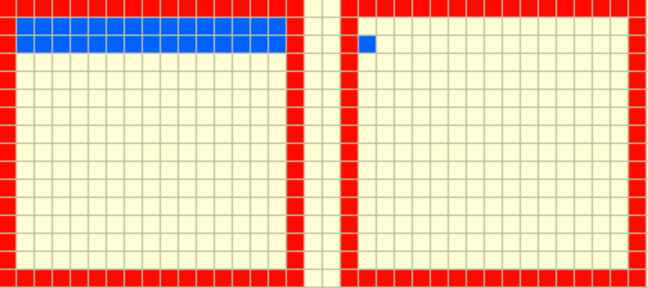
\includegraphics[scale=0.30]{figures/lu1a}\hspace{1em}
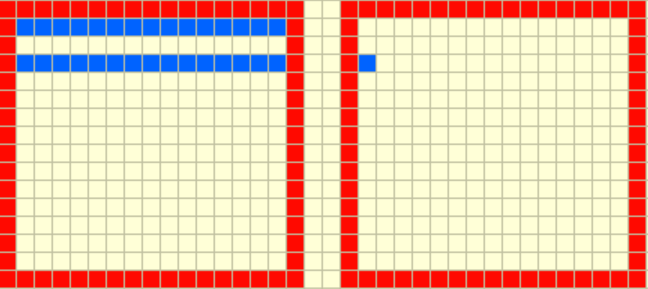
\includegraphics[scale=0.30]{figures/lu1b}
\hspace{1em}
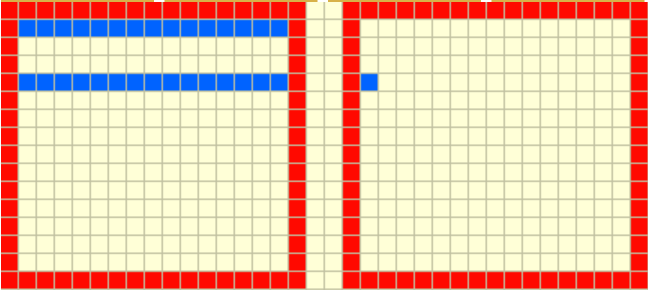
\includegraphics[scale=0.30]{figures/lu1c}
\hspace{1em}
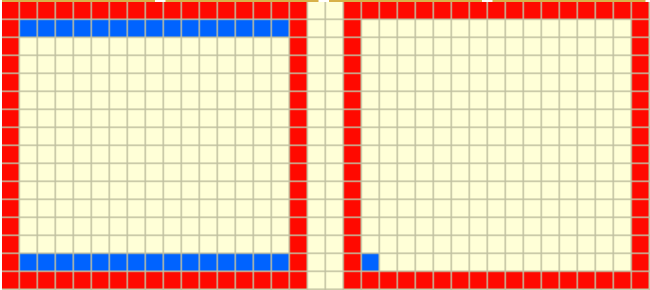
\includegraphics[scale=0.30]{figures/lu2} 


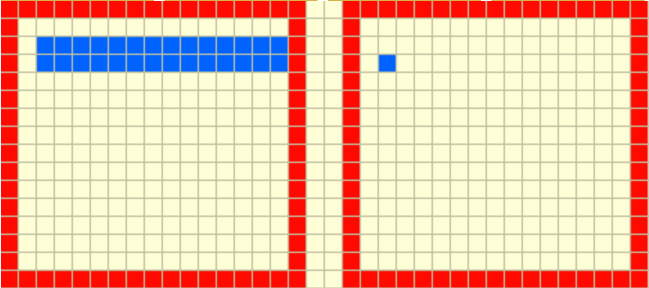
\includegraphics[scale=0.30]{figures/lu3}
\hspace{1em}
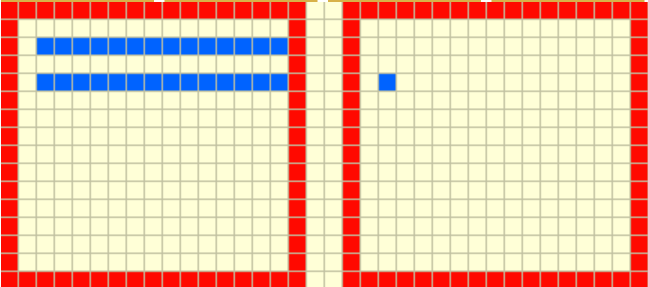
\includegraphics[scale=0.30]{figures/lu4}
\hspace{1em}
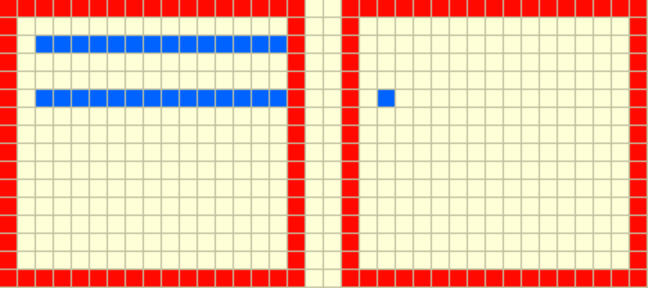
\includegraphics[scale=0.30]{figures/lu2b}
\hspace{1em}
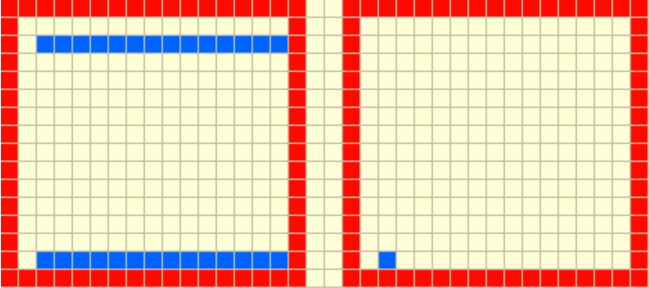
\includegraphics[scale=0.30]{figures/lu5}
$$\vdots$$
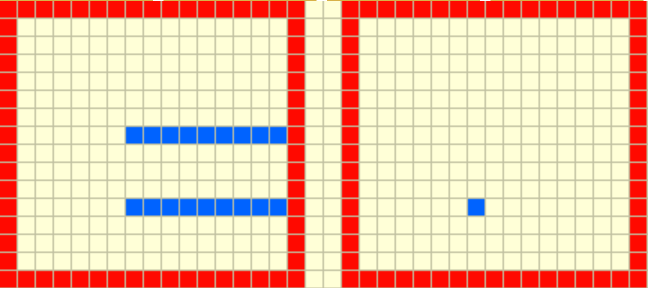
\includegraphics[scale=0.33]{figures/lu6}
$$\vdots$$
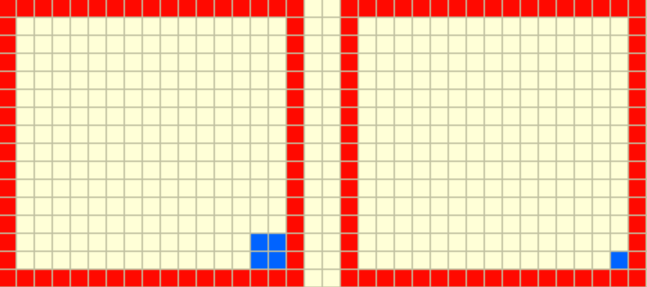
\includegraphics[scale=0.33]{figures/lu7}
\end{center}

In future work, we would like to use this access pattern to optimize the program for a particular cache configuration.

\section{Existing Work}

Many implementations of the parallelizing a LU Factorization have been attempted recently. At the 13th IEEE International Conference on Computational Science and Engineering, a group from Greece presented a parallelization using a pipelining technique in an OpenMP programming environment. They did this using coordinating threads with the help of an array of queues.  Another study done at NJIT parallelized by focusing on the load balancing techniques to translate hardware parallelization into high speedups on real applications by ordering the matrices into BDB for and eliminating data dependencies and communication during the factorization. 

\section{Approach}

We will start off with a simple implementation of LU factorization that is not optimized for any particular architecture which will serve as a starting point to measure performance improvements.


\subsection{Architecture}

Our initial optimizations target a multicore CPU architecture, such as the current Intel Haswell series i7 4970K processor. By utilizing OpenMP, our code will be accessible on a wide variety of platforms. This project may also utilize CUDA in order to implement parallel optimizations on the GPU. GPU parallelization is advantageous as it allows us to take advantage of a large number of cores + threads. Code optimizations will target the most recent nvidia GTX 970 GPU. 

\subsection{Optimizations}

We will use many well known optimization techniques to speed up our program.  In addition to the standard optimizations at the -O1, -O2, and -O3 levels, we will incorporate loop unrolling, vectorization, and parallelism.  Technically, vectorization is done automatically at the -O3 level by default, but we will apply it at the -O2 level to determine the impact it had on our code base.  All other optimizations will be applied at the -O3 level.  Additionally, we will use the -march=native compiler flag to let gcc make architecture specific optimizations.  We apply these optimizations using compiler flags and compiler hints in the code via the use of \#pragma's.  All optimations will be tested in sequence (each new optimization is added to the previous set of optimizations):

\begin{center}
\begin{tabular}{|l|l|}
\hline
Optimization & Compile Settings \\
\hline
None & gcc -o lu -std=c99 lu.c \\
-O1 & gcc -o lu -O1  -std=c99 lu.c	 \\
-O2 & gcc -o lu -O2 -std=c99 lu.c \\
Vectorization & gcc -o lu -O2 -ftree-vectorize -std=c99 lu.c \\
-O3 & gcc -o lu -O3 -std=c99 lu.c	 \\
Unroll & gcc -o lu -O3 -std=c99 -funroll-loops lu.c \\
Native Opts & gcc -o lu -O3 -std=c99 -funroll-loops -march=native lu.c \\
openMP (2 Threads) & gcc -o lu -O3 -std=c99 -fopenmp -funroll-loops -march=native lu.c \\
openMP (4 Threads) & gcc -o lu -O3 -std=c99 -fopenmp -funroll-loops -march=native lu.c \\
openMP (8 Threads) & gcc -o lu -O3 -std=c99 -fopenmp -funroll-loops -march=native lu.c \\
\hline
\end{tabular}
\end{center}

\subsection{Benchmarking}

We will evaluate the efficiency of the different optimizations using wall clock time as the performance metric.  For each optimization, we will run a benchmarking function for that program that runs the LU decomposition algorithm for matrices of size $100,200,400,800,1600,3200,6400$.  The matrices that we use will be dense where each entry is a random floating point number.  While random matrices aren't commonly used in practice, the number of floating point operations will end up being similar for all dense matrices of the same size.  Finally, for each matrix size, we will run $4$ trials to reduce the variance of the measurements.

\section{Results}

Our optimizations made a significant impact on runtimes; our best configuration settings  yielded more than 10x speedup for the large matices.  Here is the full table of data we collected:

\hskip-2.2cm
\begin{tabular}{|c|c|c|c|c|c|c|c|c|c|c|}
\hline
n & None & -O1 & -O2 & Vector & -O3 & Unroll & Native & 2 Threads & 4 Threads & 8 Threads\\
\hline
100	& 0.002791 & 0.000985 & 0.000722 & 0.000486 & 0.000509 & 0.000435 & 0.000338 & 	0.000337 & 0.001492	& 0.000409 \\
200	& 0.010098 & 0.003421 &	0.002578 &	0.00174 & 0.00176 & 0.002456 & 0.001417 & 	0.0014 & 0.000963 &	0.000725 \\
400	& 0.079022 & 0.021911 & 0.018938 & 0.015761 & 0.015605 & 0.015062 & 0.012435 & 0.006679 & 0.003321 & 0.002973 \\
800	& 0.622243 & 0.157513 & 0.10749 & 0.085002 & 0.082096 & 0.080036 & 0.066184 & 0.036134 & 0.02161 & 0.021725 \\
1600 & 4.936436 & 1.334268 & 0.938765 & 0.773718 & 0.790041 & 0.746496 & 0.6732 &	0.354768 & 0.221714 & 0.219362 \\
3200&39.711475&11.7545&9.555769&8.460412&	8.415669&8.136284&8.05138&4.457911&3.46599&	3.567894 \\

6400&316.28476&94.23317&78.119026&	69.347786&68.696747&66.535667&66.760086&	36.836628&28.870047&30.108377 \\
\hline
\end{tabular}

A few take aways from this data:

\begin{itemize}
\setlength\itemsep{0.25em}
\item Going from no optimizations to -O1 gave nearly 400\% speedup.  
\item Vectorization yielded an 11\% speedup.
\item Loop unrolling gave a 3 \% speedup in the largest case.
\item Native optimizations (-march=native) yieled a 15 \% speedup in the best case (n = 1600).  
\item From 1 core to 2 cores, we achieved a scalability of 1.81. 
\item Past 2 cores, we saw diminishing returns.  
\end{itemize}

Here are some graphs that show our results, broken up by relevant parameters.  

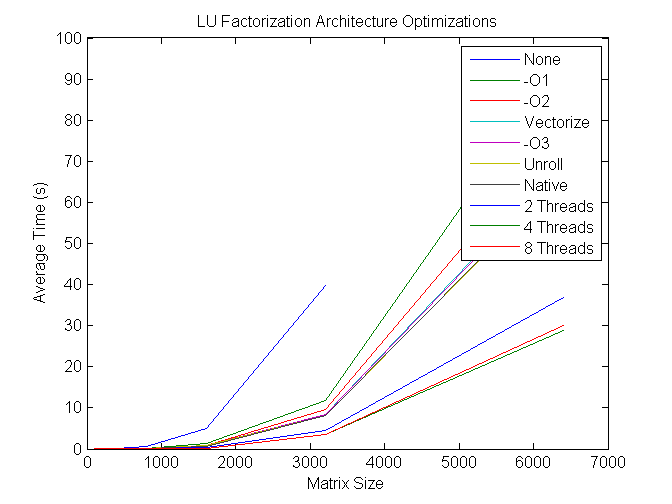
\includegraphics[scale=1]{figures/fig1}

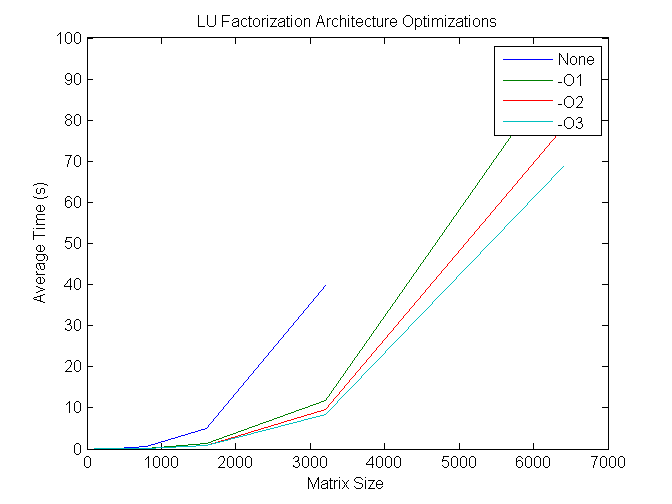
\includegraphics[scale=0.5]{figures/fig2}
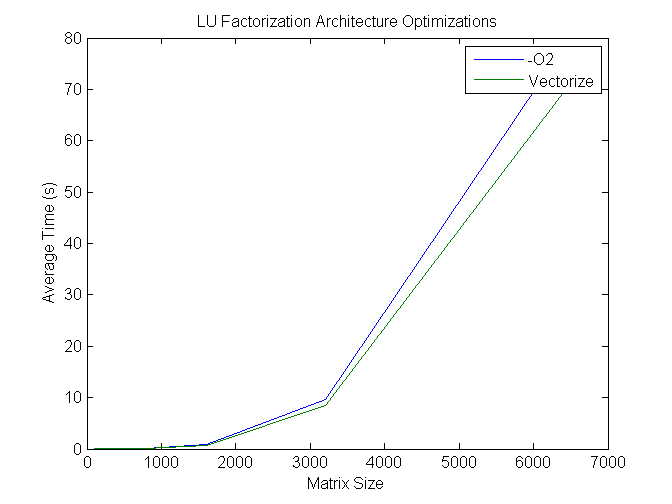
\includegraphics[scale=0.5]{figures/fig3}

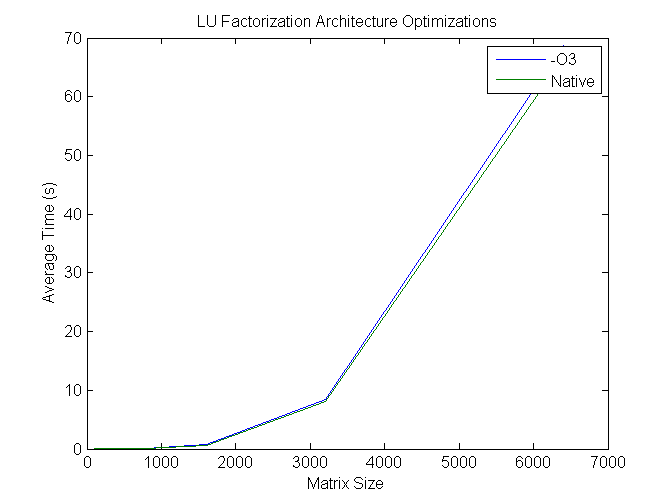
\includegraphics[scale=0.5]{figures/fig4}
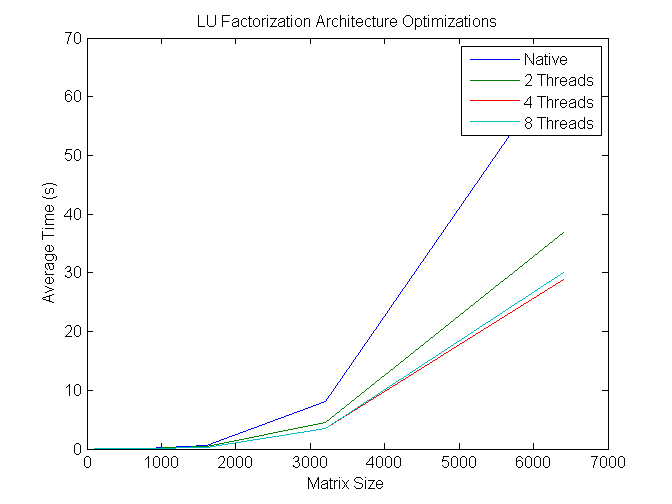
\includegraphics[scale=0.5]{figures/fig5}

\section{Conclusion}

By understanding and optimizing for the architecture we were running on, we were able to extract the maximum performance out of our program.  Each of the optimizations we used were very simple to add into our existing code base, and we didn't need to sacrifice code readability and modularity in exchange for performance.  Each optimization was either a compiler hint in the form of a \#pragma, or a compiler flag. 

Without any work at all, compiling with -O3 gave us a 4.6 x speedup.  With a little extra work, were were able to harness four cores on the computer using openMP; this yielded an 11 x.  It appeared that there were diminshing returns as more cores were introduced, which seems to limit the size of matrices computational mathemiticians can work with.  Fortunately, a 6400 x 6400 matrix is more than big enough for most applications.   

\end{document}